\documentclass[aspectratio=169,10pt]{beamer}

\usepackage[T1]{fontenc}
\usepackage{lmodern}
\usepackage{amsmath}
\usepackage{booktabs}
\usepackage{graphicx}
\usepackage{xcolor}
\usepackage{tikz}
\usetikzlibrary{positioning}

\definecolor{CDetBlue}{HTML}{17365D}
\definecolor{CDetLightBlue}{HTML}{DCEAF7}
\definecolor{CDetOrange}{HTML}{D97706}
\definecolor{CDetGray}{HTML}{4B5563}
\definecolor{CDetGreen}{HTML}{287A52}

\usetheme{default}
\usefonttheme{professionalfonts}
\setbeamercolor{normal text}{fg=black,bg=white}
\setbeamercolor{structure}{fg=CDetBlue}
\setbeamercolor{frametitle}{fg=white,bg=CDetBlue}
\setbeamercolor{title}{fg=white}
\setbeamercolor{subtitle}{fg=CDetLightBlue}
\setbeamercolor{alerted text}{fg=CDetOrange}
\setbeamertemplate{navigation symbols}{}
\setbeamertemplate{itemize item}{\color{CDetOrange}$\blacktriangleright$}
\setbeamertemplate{itemize subitem}{\color{CDetBlue}$\bullet$}
\setbeamertemplate{frametitle}{%
  \nointerlineskip
  \begin{beamercolorbox}[wd=\paperwidth,ht=0.78cm,dp=0.22cm,leftskip=0.48cm]{frametitle}
    \usebeamerfont{frametitle}\insertframetitle
  \end{beamercolorbox}}
\setbeamertemplate{footline}{%
  \leavevmode
  \hbox{%
    \begin{beamercolorbox}[wd=.82\paperwidth,ht=0.28cm,dp=0.14cm,leftskip=0.45cm]{author in head/foot}%
      \color{CDetGray}\scriptsize CDet cross-target timing calibration, run 5710
    \end{beamercolorbox}%
    \begin{beamercolorbox}[wd=.18\paperwidth,ht=0.28cm,dp=0.14cm,rightskip=0.45cm plus1fil]{date in head/foot}%
      \color{CDetGray}\scriptsize\hfill\insertframenumber/\inserttotalframenumber
    \end{beamercolorbox}}}
\setbeamersize{text margin left=0.55cm,text margin right=0.55cm}

\newcommand{\result}[1]{\textcolor{CDetGreen}{\textbf{#1}}}
\newcommand{\lesson}[1]{\textcolor{CDetOrange}{\textbf{#1}}}
\newcommand{\code}[1]{\texttt{\small #1}}

\title{CDet timing calibration with cross-target run 5710}
\subtitle{A start-to-finish account of the procedure, failures, and final closure}
\author{CDet group meeting}
\date{September 2026}

\begin{document}

\begin{frame}[plain]
  \begin{tikzpicture}[remember picture,overlay]
    \fill[CDetBlue] (current page.south west) rectangle (current page.north east);
    \fill[CDetOrange] (current page.south west) rectangle ([xshift=0.16cm]current page.north west);
  \end{tikzpicture}
  \vspace{1.4cm}
  {\usebeamerfont{title}\color{white}\LARGE\bfseries\inserttitle\par}
  \vspace{0.45cm}
  {\color{CDetLightBlue}\large\insertsubtitle\par}
  \vfill
  {\color{white}\insertauthor\par}
  {\color{CDetLightBlue}\insertdate\par}
  \vspace{0.5cm}
\end{frame}

\begin{frame}{Calibration target and data set}
\begin{columns}[T,onlytextwidth]
  \column{0.55\textwidth}
  \begin{itemize}
    \item Cross-target run \textbf{5710}
    \item \textbf{2,951,891} available events
    \item Two CDet layers, each containing 84 half-bars
    \item 2,688 logical pixel/channel IDs
    \item ECal provides event selection, position matching, and the timing reference
  \end{itemize}
  \vspace{0.25cm}
  \lesson{Goal:} align usable pixels and half-bars near 30 ns while removing ECal-time and ToT dependence.

  \column{0.41\textwidth}
  \begin{block}{Final observable}
    Accepted Layer-1/Layer-2 pairs use
    \[
      t_{\mathrm{pair}}=\frac{t_{L1}+t_{L2}}{2}.
    \]
    Its detector-wide width measures the timing performance relevant to paired hits.
  \end{block}
\end{columns}
\end{frame}

\begin{frame}{The correction model}
\small
\begin{align*}
t_{\mathrm{raw},i} &= 0.01\,t_{\mathrm{TDC},i}-t_{\mathrm{reference}},\\[1mm]
t_{\mathrm{pixel},i} &= t_{\mathrm{raw},i}+\textcolor{red}{O_i},\\[1mm]
t_{\mathrm{ECal},i} &= t_{\mathrm{pixel},i}
-(\textcolor{red}{p_0}+\textcolor{red}{p_1}t_{\mathrm{ECal}})
+\textcolor{red}{\Delta_h},\\[1mm]
t_{\mathrm{final},i} &= t_{\mathrm{ECal},i}
-\textcolor{red}{q_{L}}\left(\frac{1}{\sqrt{\mathrm{ToT}}}
-\frac{1}{\sqrt{\mathrm{ToT}_{\mathrm{ref},L}}}\right)
+\textcolor{red}{s_{\mathrm{run}}}.
\end{align*}
\vspace{0.05cm}
\begin{columns}[T,onlytextwidth]
  \column{0.48\textwidth}
  \textbf{Local corrections}
  \begin{itemize}
    \item \textcolor{red}{$O_i$}: one offset per paddle
    \item \textcolor{red}{$\Delta_h$}: later common shift for the 16 pixels in each half-bar
  \end{itemize}
  \column{0.48\textwidth}
  \textbf{Shared corrections}
  \begin{itemize}
    \item \textcolor{red}{$p_0,p_1$}: one ECal timing pair for the entire detector
    \item \textcolor{red}{$q_L$}: one time-walk coefficient per layer
    \item \textcolor{red}{$s_{\mathrm{run}}$}: optional global timing shift for one run, read from \texttt{CDet\_run<run>.dat}. It is zero for run 5710
  \end{itemize}
\end{columns}
\end{frame}

\begin{frame}{Initial two-pass workflow}
\centering
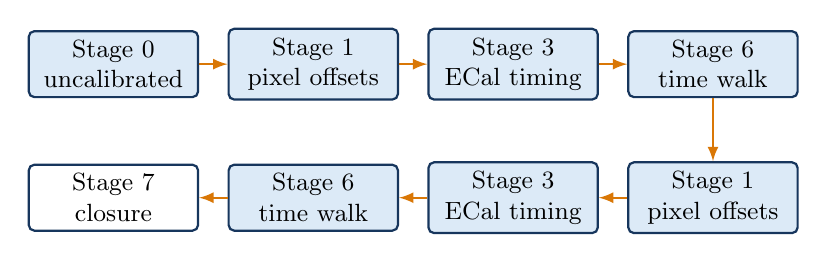
\begin{tikzpicture}[node distance=0.45cm and 0.36cm,
  box/.style={draw=CDetBlue,thick,rounded corners=2pt,fill=CDetLightBlue,
              minimum width=2.15cm,minimum height=0.72cm,align=center,font=\small},
  arr/.style={-latex,thick,CDetOrange}]
  \node[box] (s0) {Stage 0\\uncalibrated};
  \node[box,right=of s0] (s1) {Stage 1\\pixel offsets};
  \node[box,right=of s1] (s3) {Stage 3\\ECal timing};
  \node[box,right=of s3] (s6) {Stage 6\\time walk};
  \draw[arr] (s0)--(s1); \draw[arr] (s1)--(s3); \draw[arr] (s3)--(s6);
  \node[box,below=0.8cm of s6] (s1b) {Stage 1\\pixel offsets};
  \node[box,left=of s1b] (s3b) {Stage 3\\ECal timing};
  \node[box,left=of s3b] (s6b) {Stage 6\\time walk};
  \node[box,left=of s6b,fill=white] (s7) {Stage 7\\closure};
  \draw[arr] (s6)--(s1b); \draw[arr] (s1b)--(s3b); \draw[arr] (s3b)--(s6b); \draw[arr] (s6b)--(s7);
\end{tikzpicture}
\vspace{0.55cm}
\begin{itemize}
  \item Each fit adds a residual correction to the constants already loaded.
  \item The driver must load the master macro first, or compile the self-contained driver with ACLiC.
  \item Stage 7 applies pixel offsets, ECal timing, and time walk together.
\end{itemize}
\end{frame}

\begin{frame}{First correction: the pairing ToT cut}
\begin{columns}[T,onlytextwidth]
  \column{0.67\textwidth}
  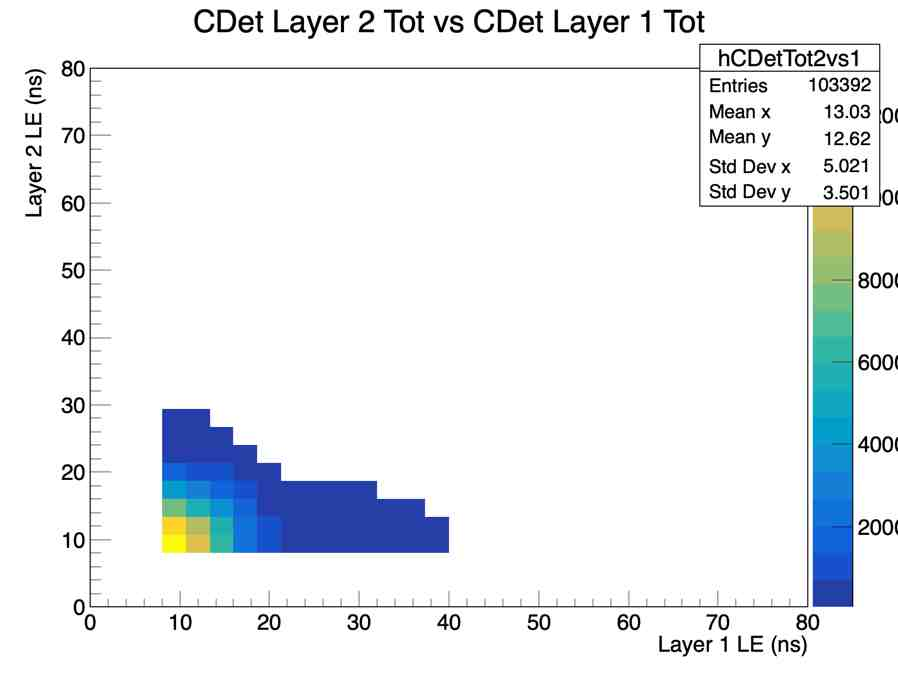
\includegraphics[width=\linewidth,height=0.74\textheight,keepaspectratio]{cCDetTotLayer2v1.jpg}
  \column{0.30\textwidth}
  The original pairing fit required
  \[
    8 < \mathrm{ToT} < 40~\mathrm{ns}.
  \]
  The lower threshold removed a visible population of otherwise useful hits.

  \vspace{0.35cm}
  We changed the pairing range to
  \[
    \textcolor{CDetGreen}{\mathbf{4 < \mathrm{ToT} < 40~\mathrm{ns}}}.
  \]

  \vspace{0.25cm}
  \lesson{Lesson:} selection cuts need visual validation at every calibration stage.
\end{columns}
\end{frame}

\begin{frame}{The pixel-fit failure was physical, not merely numerical}
\begin{columns}[T,onlytextwidth]
  \column{0.72\textwidth}
  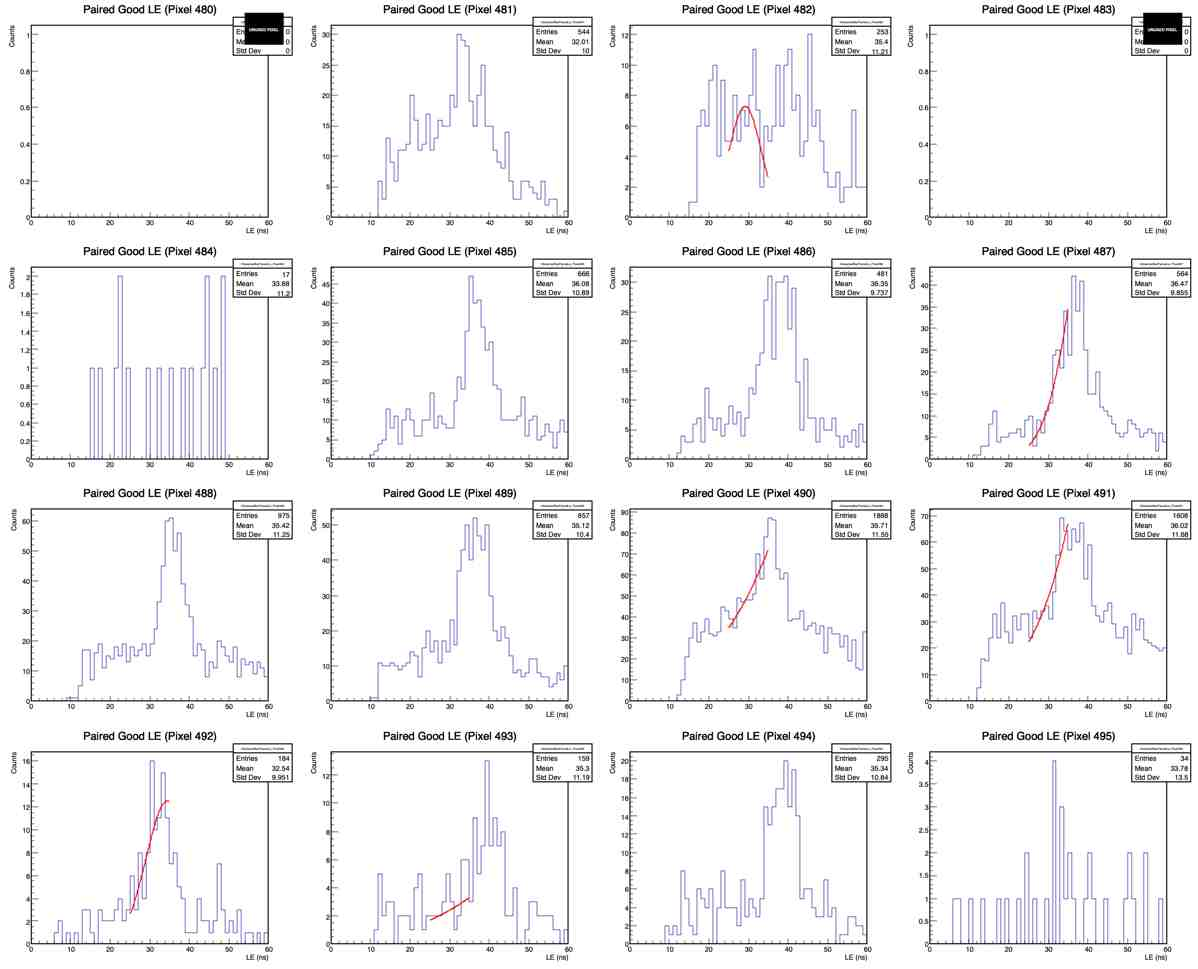
\includegraphics[width=\linewidth,height=0.78\textheight,keepaspectratio]{cSelectedBarPairedLe.jpg}
  \column{0.25\textwidth}
  Bar 29 exposed side peaks from multi-anode PMT cross-talk.

  \vspace{0.25cm}
  For pixels such as 468, the cross-talk peak could exceed the real peak. A blind fit then selected the wrong population.

  \vspace{0.3cm}
  \lesson{Largest peak} did not always mean \lesson{physical peak}.
\end{columns}
\end{frame}

\begin{frame}{Hierarchical pixel-offset extraction}
\begin{columns}[T,onlytextwidth]
  \column{0.48\textwidth}
  \textbf{Group estimate}
  \begin{itemize}
    \item Divide each 16-pixel half-bar into groups 0--7 and 8--15.
    \item Sum actual counts without per-pixel normalization.
    \item Require at least 100 group entries.
    \item Fit over $-30 < t_{\mathrm{ECal}}-t_{\mathrm{CDet}} < +10$ ns.
  \end{itemize}
  \column{0.48\textwidth}
  \textbf{Individual estimate}
  \begin{itemize}
    \item Require at least 35 pixel entries.
    \item Seed a narrow fit from the group centroid.
    \item Accept $0.5 < \sigma < 8$ ns, significance $>1.5$, and $\chi^2/\mathrm{NDF}<15$.
    \item Use the group centroid as fallback; use a broad individual fit when the group fit fails.
  \end{itemize}
\end{columns}
\vspace{0.25cm}
\begin{block}{Robust reference}
The detector reference is the median of valid individual centroids. The residual update is
\[
  O_i^{\mathrm{new}}=O_i^{\mathrm{old}}+(\mu_i-\mu_0).
\]
\end{block}
\end{frame}

\begin{frame}{Hierarchical diagnostics made every decision inspectable}
\centering

\includegraphics[width=0.93\linewidth,height=0.78\textheight,keepaspectratio]{tdcPlots/hierarchical/bar029_hierarchical.png}

\vspace{-0.1cm}
\small Group fits, individual fits, fallbacks, and retained offsets are stored together in a hierarchical ROOT file.
\end{frame}

\begin{frame}{Manual LE--ToT polygons resolved ambiguous pixels}
\begin{columns}[T,onlytextwidth]
  \column{0.52\textwidth}
  The interactive editor displays each flagged pixel in LE versus ToT and saves a \texttt{TCutG} around the physical population.

  \begin{itemize}
    \item Candidate ranking deliberately favored sensitivity over specificity.
    \item We reviewed both banks of all 84 half-bars.
    \item The final cut file contains \textbf{102 manual pixel polygons}.
  \end{itemize}

  \vspace{0.25cm}
  A manual polygon already resolves the ambiguity. Its 1D timing fit therefore uses an independent seed rather than the group centroid.

  \column{0.44\textwidth}
  \begin{block}{Important implementation detail}
    Editing polygons changes only the cut file.

    The timing constants change only after rerunning
    \begin{center}
      \resizebox{0.98\linewidth}{!}{\texttt{extractHierarchicalCDetPixelTimingOffsets(...)}}
    \end{center}
  \end{block}
  \begin{block}{Preservation rule}
    The editor updates cuts in place. Existing cuts remain intact while selected pixels are revisited.
  \end{block}
\end{columns}
\end{frame}

\begin{frame}{ECal timing: the pooled result looked reassuring}
\begin{columns}[T,onlytextwidth]
  \column{0.68\textwidth}
  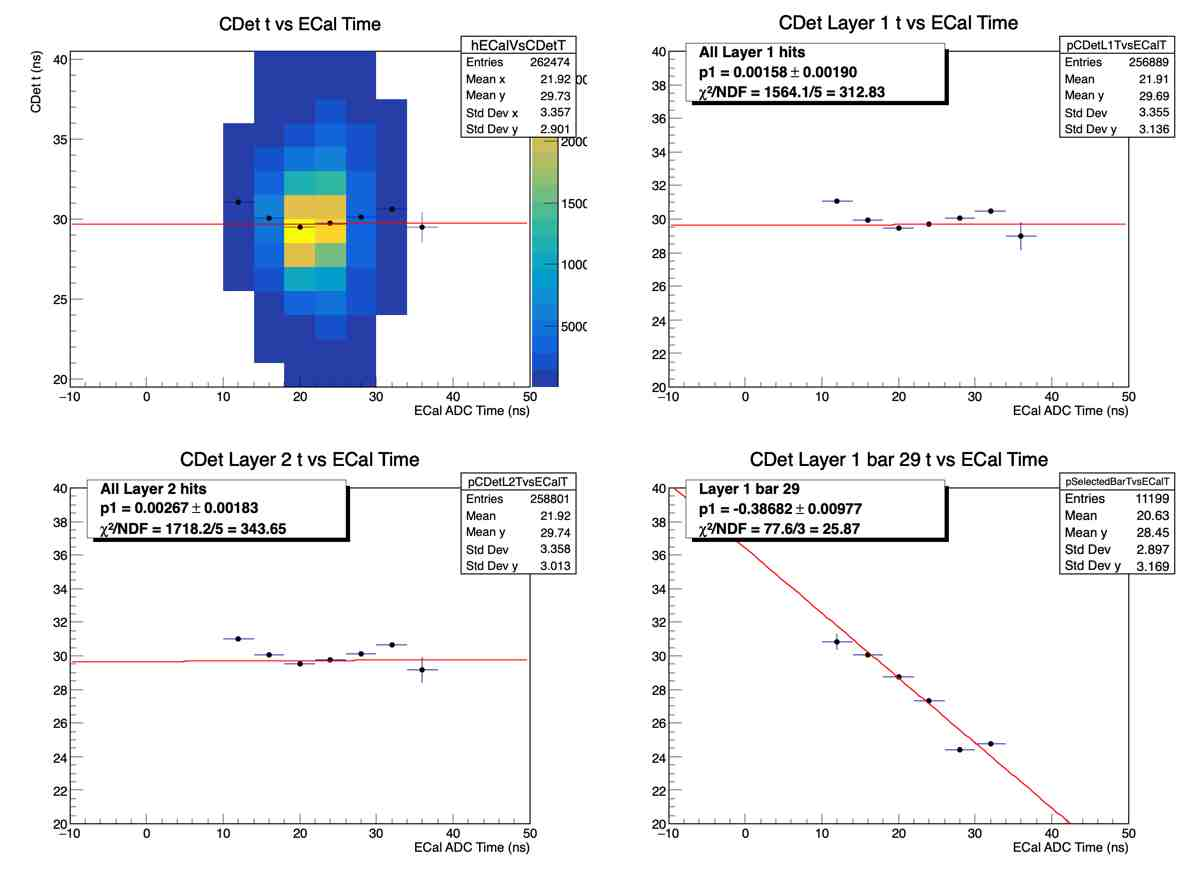
\includegraphics[width=\linewidth,height=0.74\textheight,keepaspectratio]{simpsons_paradox_run5710_before_correction/pooled_and_selected_ecal_timing_diagnostics.jpg}
  \column{0.29\textwidth}
  The pooled CDet-versus-ECal profile appeared nearly flat.

  The selected half-bar showed a strong negative slope.

  \vspace{0.4cm}
  \lesson{The aggregate fit concealed the dependence that mattered.}
\end{columns}
\end{frame}

\begin{frame}{Simpson's paradox across CDet half-bars}
\begin{columns}[T,onlytextwidth]
  \column{0.62\textwidth}
  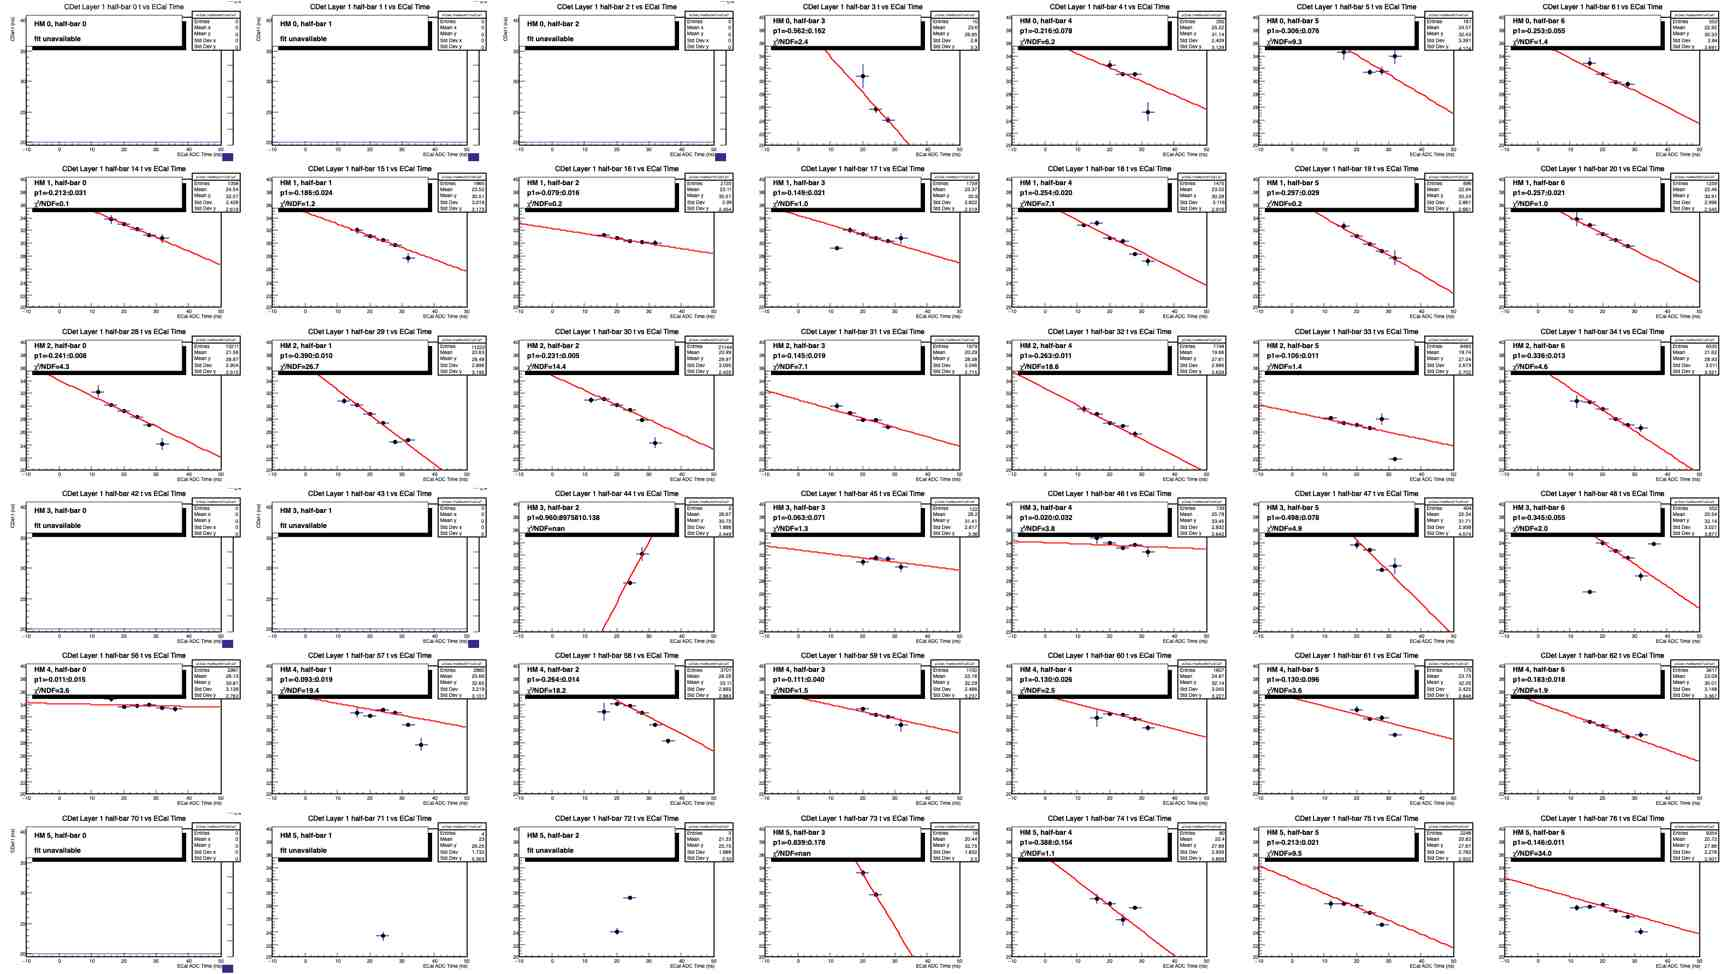
\includegraphics[width=\linewidth,height=0.72\textheight,keepaspectratio]{simpsons_paradox_run5710_before_correction/layer1_bank0_halfbar_ecal_timing.jpg}
  \column{0.35\textwidth}
  Of 135 fitted half-bars:
  \begin{itemize}
    \item 130 slopes were negative.
    \item 122 were negative by more than $2\sigma$.
    \item Mean slope: $-0.1284$ ns/ns.
  \end{itemize}

  \vspace{0.15cm}
  Yet the pooled profile remained nearly flat because positive covariance among half-bar means cancelled the negative within-half-bar covariance.

  \vspace{0.25cm}
  \lesson{This was a detector-calibration example of Simpson's paradox.}
\end{columns}
\end{frame}

\begin{frame}{Fixed effects isolated the physical ECal dependence}
\begin{columns}[T,onlytextwidth]
  \column{0.49\textwidth}
  For hit $j$ in half-bar $h$, center both variables within that half-bar:
  \[
    x_{hj}=t_{\mathrm{ECal},hj}-\overline{t}_{\mathrm{ECal},h},
  \]
  \[
    y_{hj}=t_{\mathrm{CDet},hj}-\overline{t}_{\mathrm{CDet},h}.
  \]
  Fit one unbinned common slope to $(x_{hj},y_{hj})$ while allowing every half-bar its own intercept.

  \column{0.48\textwidth}
  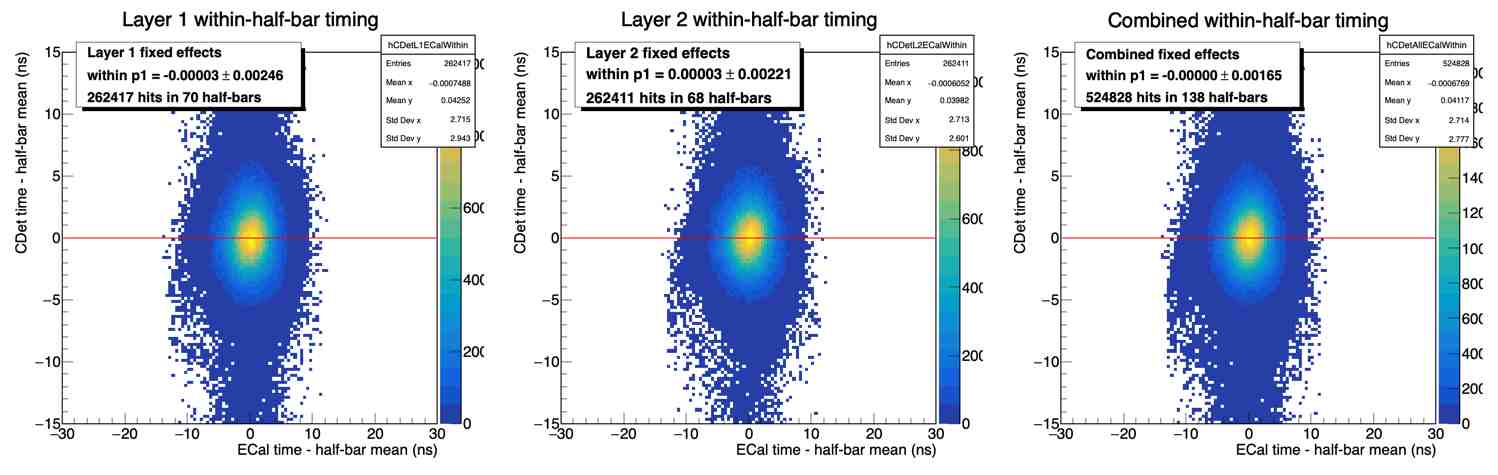
\includegraphics[width=\linewidth,height=0.64\textheight,keepaspectratio]{CDet_run5710_fixed_effects_final_archive/CDet_ECal_fixed_effects_final_closure.jpg}
\end{columns}
\vspace{0.2cm}
\result{The combined fixed-effects slope, not the pooled profile slope, became the calibration estimator.}
\end{frame}

\begin{frame}{ECal-slope closure}
\centering

\includegraphics[width=0.93\linewidth,height=0.68\textheight,keepaspectratio]{CDet_run5710_halfbar_aligned_final_archive/CDet_ECal_fixed_effects_final_closure.jpg}

\vspace{0.1cm}
\begin{tabular}{lrr}
\toprule
Sample & Residual slope (ns/ns) & Statistical uncertainty \\
\midrule
Layer 1 & $+0.000743$ & $0.002474$ \\
Layer 2 & $-0.000738$ & $0.002216$ \\
Combined & $+0.000000028$ & $0.001660$ \\
\bottomrule
\end{tabular}
\end{frame}

\begin{frame}{A flat slope did not guarantee detector-wide alignment}
\begin{columns}[T,onlytextwidth]
  \column{0.52\textwidth}
  After removing the common ECal slope, half-bars still had different intercepts at the same ECal reference time.

  \begin{itemize}
    \item Reference time: $t_{\mathrm{ECal}}=22$ ns
    \item Validated half-bars: 123 of 168
    \item Detector reference: 29.6304 ns
    \item Between-half-bar RMS before alignment: 1.61545 ns
  \end{itemize}

  \column{0.44\textwidth}
  Each accepted half-bar received one common additive increment across its 16 pixels:
  \[
    \delta O_h=t_{\mathrm{reference}}-t_h(22~\mathrm{ns}).
  \]
  This preserves the within-half-bar ECal slope and the relative pixel structure.
\end{columns}
\end{frame}

\begin{frame}{Half-bar intercept closure}
\centering
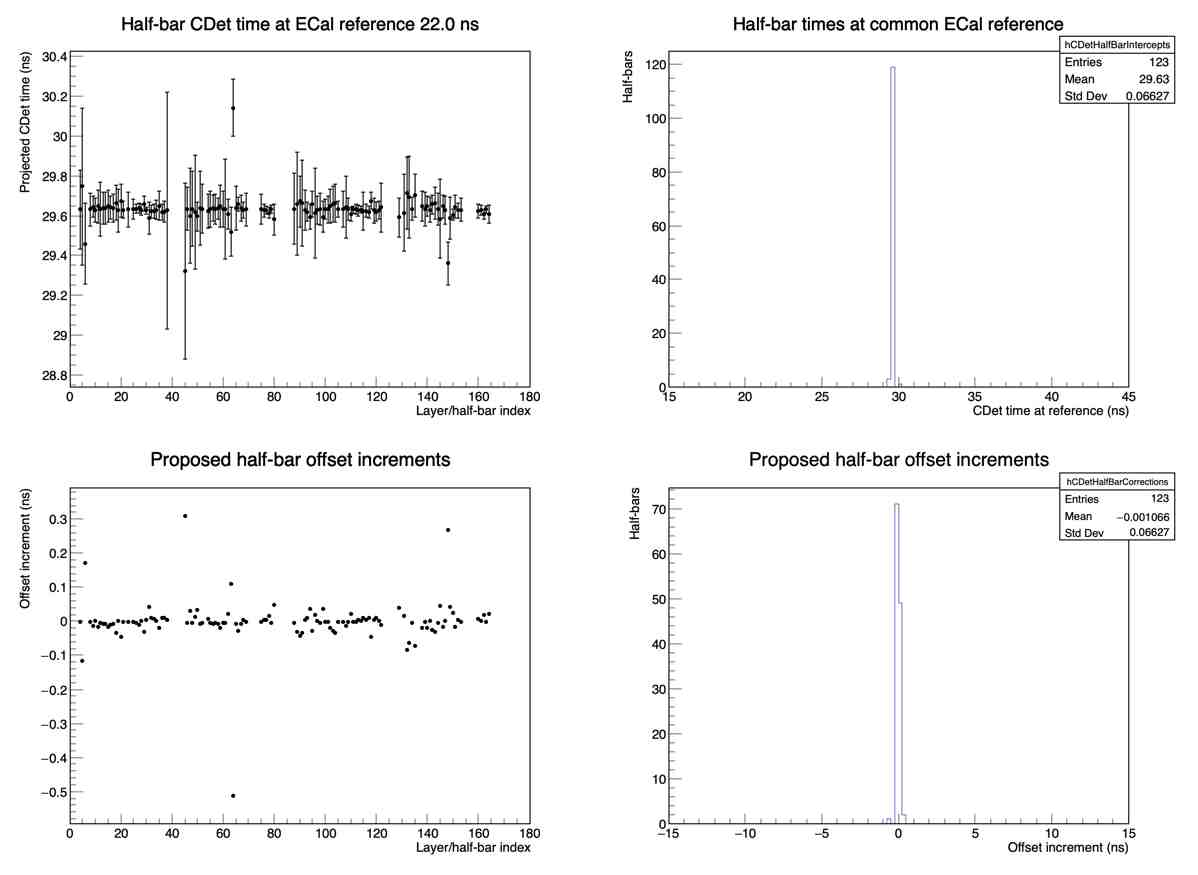
\includegraphics[width=0.94\linewidth,height=0.79\textheight,keepaspectratio]{CDet_run5710_halfbar_aligned_final_archive/CDet_halfbar_intercept_final_closure.jpg}
\end{frame}

\begin{frame}{Final calibrated timing}
\begin{columns}[T,onlytextwidth]
  \column{0.49\textwidth}
  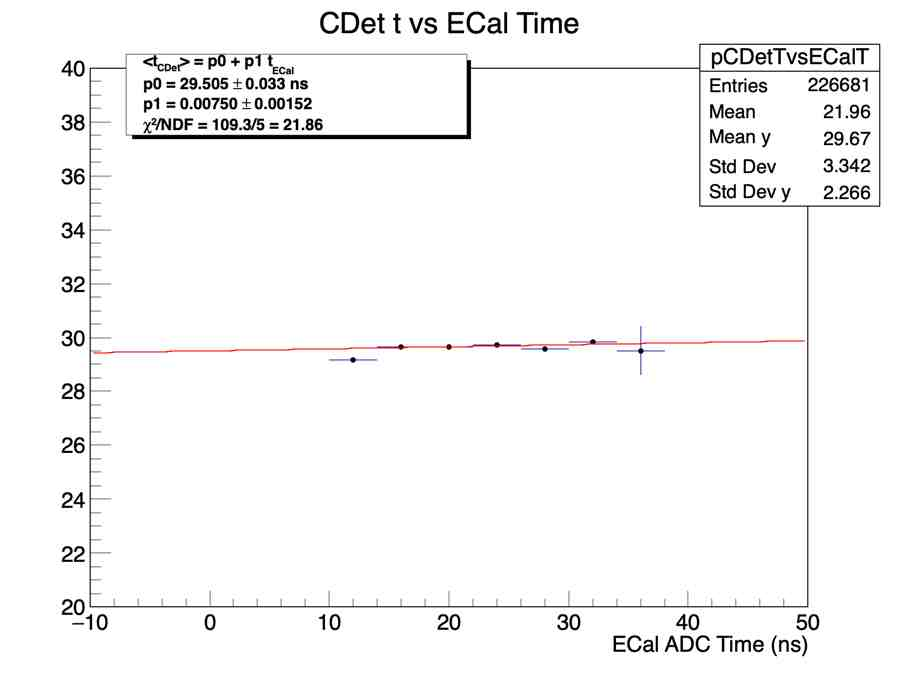
\includegraphics[width=\linewidth,height=0.64\textheight,keepaspectratio]{CDet_run5710_halfbar_aligned_final_archive/CDet_pooled_timing_final.jpg}
  \column{0.48\textwidth}
  \textbf{Final constants}
  \[
    p_0=74.192800~\mathrm{ns},\qquad p_1=0.817261.
  \]
  \begin{itemize}
    \item Between-half-bar RMS: \result{0.03961 ns}
    \item Individual-hit RMS: \result{2.99623 ns}
    \item Paired-layer mean-time width: \result{$\approx 2.27$ ns}
    \item Predicted gain from another alignment: only 0.00026 ns
  \end{itemize}
  \vspace{0.2cm}
  The large change in $p_0$ relative to the older calibration agrees qualitatively with the ECal group's roughly 100 ns database timing shift.
\end{columns}
\end{frame}

\begin{frame}{What we learned}
\begin{itemize}
  \item Cross-talk can make the largest 1D timing peak the wrong physical population. LE--ToT information resolves that ambiguity.
  \item Group fits help seed sparse pixels, but real counts must remain unnormalized and group-fit $\chi^2$ should remain diagnostic.
  \item Manual polygons should bypass the group-centroid constraint because the user has already identified the physical population.
  \item A pooled timing slope can hide strong within-detector trends. Half-bar fixed effects provide the relevant ECal correction.
  \item Removing a common slope and aligning half-bar intercepts solve different problems. Both steps matter for detector-wide resolution.
  \item Every automated update needs a diagnostic-only mode, preserved inputs, auditable fit results, and a final closure run.
\end{itemize}
\end{frame}

\begin{frame}{Definitive run-5710 products}
\small
The final archive is
\[
\texttt{CDet\_run5710\_halfbar\_aligned\_final\_archive/}.
\]
It contains:
\begin{itemize}
  \item the definitive calibration file;
  \item the 102 manual LE--ToT polygon cuts;
  \item hierarchical pixel-fit results and ROOT diagnostics;
  \item applied half-bar increments and final closure records;
  \item final pooled, fixed-effects, and intercept-alignment figures;
  \item SHA-256 checksums for the primary artifacts.
\end{itemize}
\vspace{0.25cm}
\begin{block}{Repository checkpoint}
Tag: \texttt{cdet-run5710-halfbar-aligned-final-v2.0}
\end{block}
\end{frame}

\appendix

\begin{frame}[fragile]{Appendix: full calibration command}
\scriptsize
\begin{verbatim}
.L PlotElastic_Calibration_Master_stageflag_singlefile_crosstarget.C+
.L Run_CDet_Calibration_TwoPass_InSession_AllCross_Individually.C

Run_CDet_Calibration_TwoPass_InSession_AllCross_Individually(
    5710, -1, 0, -1, -1,
    0.02, 60, 4, 50,
    1, 100, 1, 100,
    0.10, 0.02, 0.1,
    3, false, 30, 2, 1, true);
\end{verbatim}
\vspace{0.25cm}
The final \texttt{true} removes the active calibration and starts fresh. Back up
\texttt{CDet\_calibration\_dt.dat} before using it.
\end{frame}

\begin{frame}[fragile]{Appendix: validation and resolution}
\scriptsize
\begin{verbatim}
.L PlotElastic_Calibration_Master_stageflag_singlefile_crosstarget.C+

PlotElastic_Calibration_Master_stageflag_singlefile_crosstarget(
    "CDet_run5710_event_display.conf");

plotCDetLayersTimeComp("CDet_run5710_event_display.conf");

reportCDetPairedTimeResolution();
\end{verbatim}
\vspace{0.25cm}
The resolution helper reports the RMS of the full accepted-pair mean-time
distribution separately from a Gaussian fit to its central 25--35 ns core.
\end{frame}

\end{document}
